% LICENSE: see LICENCE
\RequirePackage[l2tabu, orthodox]{nag}
\nonstopmode
\documentclass[a4paper,oneside,10pt]{article}

%include version control info
\input{vc.tex}

%\usepackage[bindingoffset=1.5cm,centering,includeheadfoot,margin=3cm]{geometry}

\usepackage[T1]{fontenc}
\usepackage[utf8]{inputenc}
\usepackage[pdftex]{graphicx}
%\usepackage{subfig}

\usepackage[protrusion=true,expansion=true]{microtype}

\usepackage{wrapfig}
\usepackage{fancybox}
\usepackage{shadow}
\usepackage{xspace}
\usepackage{acronym}

%\usepackage{lmodern} % new latin extended computer modern font}, use with T1
%\usepackage{pxfonts} % has replaced palatino
\usepackage{cmbright}

\usepackage{listings}

\usepackage[allowlitunits]{siunitx}
% Try $20\micro\seconds$

%\addtolength{\oddsidemargin}{-1cm}
%\addtolength{\evensidemargin}{-1cm}
%\addtolength{\textwidth}{+2cm}
%\usepackage{showframe}
%\usepackage{lastpage}
% for \pageref{LastPage}

% fancy header
\usepackage{fancyhdr}
\pagestyle{fancy}
\fancyhf{} % clear default header and footer
\fancyhead[R]{\textit{\nouppercase{\leftmark}}}
\fancyhead[C]{}
\fancyfoot[R]{\thepage}
\fancyfoot[L]{\tiny{rev~\GITAbrHash, \GITAuthorDate, \GITAuthorName.}}

\setlength{\headheight}{14pt}

\newcommand\Hrule{\noindent\rule{\linewidth}{1.5pt}}
\newcommand{\sidenote}[1]{\marginpar{\scriptsize{\textsf{#1}}}} % Bram's sidenote for comments

%\usepackage{titlesec}

\newcommand{\footnoteurl}[1]{\footnote{\url{#1}}}
\newcommand{\us}{\,\si{\micro\second}\xspace}
\newcommand{\km}{\,\si{\kilo\meter}\xspace}
\newcommand{\ms}{\,ms}
\newcommand{\dabplus}{DAB$^\mathrm{+}$\xspace}
\newcommand{\captionwidth}{0.9\textwidth}
\newcommand{\mmbtools}{\mbox{ODR-mmbTools}\xspace}

\newcommand{\filename}[1]{\texttt{#1}}

% index stuff
\usepackage{tocbibind} % Index in TOC
%\usepackage{makeidx}
%\usepackage{showidx} % show index entries in margin
%\makeindex

%\newcommand{\bib}[4]{\item{\textsc{#1}, \emph{#2}, #3\\\hspace{2em}#4}}

% ---------------------------------------------------------

\newcommand{\titleinfo}{ODR-mmbTools \\
Open-Source Software-Defined \dabplus Tools}
\author{Matthias P. Brändli}
\title{\titleinfo}


% Margins for handwritten notes
%\addtolength{\oddsidemargin}{-2cm}
%\addtolength{\evensidemargin}{-2cm}
%\addtolength{\textwidth}{-2cm}

\usepackage{xcolor}
\definecolor{Brown}{cmyk}{0,0.81,1,0.60}
\definecolor{OliveGreen}{cmyk}{0.64,0,0.95,0.40}
\definecolor{CadetBlue}{cmyk}{0.62,0.57,0.23,0}
\definecolor{lightlightgray}{cmyk}{0,0,0,0.02}
\definecolor{gray}{cmyk}{0,0,0,0.8}

\usepackage{smartdiagram}

\usepackage[pdftex,
 pdfauthor={Matthias P. Braendli},
 pdftitle={ODR-mmbTools Documentation},
 pdfsubject={},
 pdfkeywords={Digital Audio Broadcasting,DAB,single-frequency network,SFN,mmbTools,ODR-mmbTools,open-source,software-defined radio},
 pdfcreator=pdflatex]{hyperref}
\hypersetup{colorlinks, citecolor=black, filecolor=black, linkcolor=black, urlcolor=black}

% LaTeX magic: make sections have a cleardoublepage
% Useful for twoside only
%\let\stdsection\section
%\renewcommand*\section{\cleardoublepage\stdsection}

\begin{document}
\lstset{
language=C,                             % Code langugage
basicstyle=\ttfamily,                   % Code font, Examples: \footnotesize, \ttfamily
keywordstyle=\color{OliveGreen},        % Keywords font ('*' = uppercase)
commentstyle=\color{gray},              % Comments font
numbers=left,                           % Line nums position
numberstyle=\tiny,                      % Line-numbers fonts
stepnumber=1,                           % Step between two line-numbers
numbersep=5pt,                          % How far are line-numbers from code
backgroundcolor=\color{lightlightgray}, % Choose background color
frame=none,                             % A frame around the code
tabsize=2,                              % Default tab size
captionpos=b,                           % Caption-position = bottom
breaklines=true,                        % Automatic line breaking?
breakatwhitespace=false,                % Automatic breaks only at whitespace?
showspaces=false,                       % Dont make spaces visible
showtabs=false,                         % Dont make tabls visible
morekeywords={uint32_t,uint8_t,uint16_t,time_spec_t,size_t,
clock_config_t},
}
\pagestyle{empty}
\pagenumbering{roman}
 \begin{titlepage}
    \null\vfil
    \begin{flushleft}
      \huge \textbf{\titleinfo}
    \end{flushleft}
    \par
    \hrule height 4pt
    \par
    \begin{flushright}
      \large
      \textsl{Project Documentation} \par
    \end{flushright}
    \vspace{\fill}
    \vspace*{\stretch{1}}

    \begin{center}
        \Large
        Opendigitalradio\\\href{http://opendigitalradio.org}{http://opendigitalradio.org}\\2014--2017
    \end{center}
    \vspace{\fill}
    \vspace*{\stretch{2}}

    \begin{figure}[!h]
        \centering
        \parbox{2.2in}{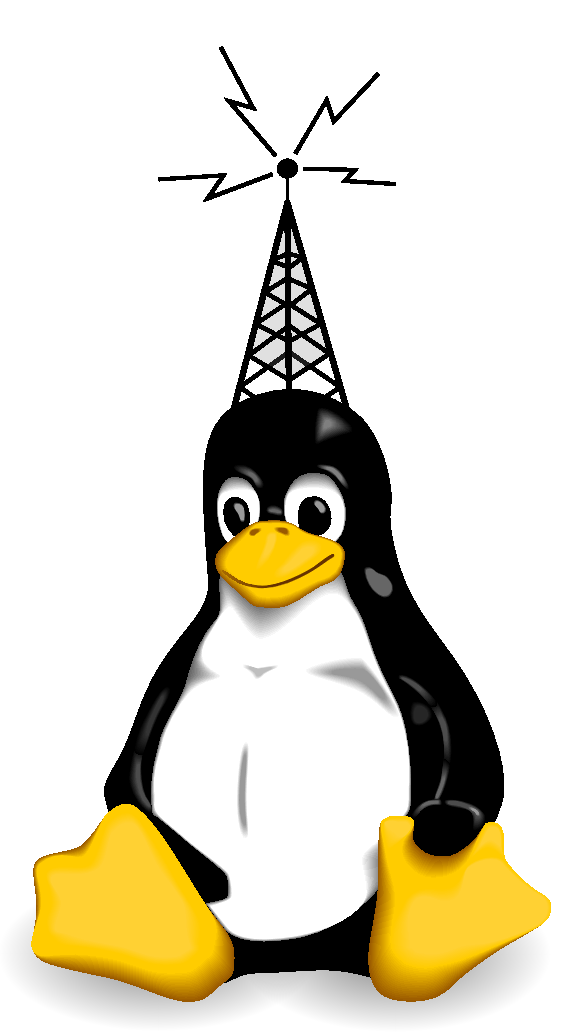
\includegraphics[width=16em]{figures/dabtux.pdf}}
    \end{figure}

    \vspace*{1cm}
    \begin{center}
    This work is licensed under a \\
    Creative Commons Attribution-ShareAlike 4.0 International License.\\
    See \url{http://creativecommons.org/licenses/by-sa/4.0/} or LICENCE.txt
    \end{center}
 \end{titlepage}

\pagestyle{fancy}
\tableofcontents

\section*{Acronyms}
\markboth{Acronyms}{}
\addcontentsline{toc}{section}{Acronyms}
\begin{acronym}[mmbTools]
    \acro{1PPS}{One pulse per second}
    \acro{CIF}{Common Interleaved Frame}
    \acro{CRC}{Communications Research Centre Canada}
    \acro{DAB}{Digital Audio Broadcasting}
    \acro{DMB}{Digital Multimedia Broadcasting}
    \acro{ETI}{Ensemble Transport Interface}
    \acro{ETSI}{European Telecommunications Standards Institute}
    \acro{FIC}{Fast Information Channel}
    \acro{HE-AAC}{High Efficiency Advanced Audio Codec}
    \acro{mmbTools}{Mobile Multimedia Broadcasting Tools}
    \acro{MNSC}{Multiplex Network Signalling Channel}
    \acro{NTP}{Network Time Protocol}
    \acro{OCXO}{Oven-Controlled Crystal Oscillator}
    \acro{OFDM}{Orthogonal Frequency-Division Multiplexing}
    \acro{PRBS}{Pseudo-Random Bit Sequence}
    \acro{SFN}{Single-Frequency Network}
    \acro{TCXO}{Temperature-Compensated Crystal Oscillator}
    \acro{TIST}{Timestamp field in the ETI frame}
    \acro{TM}{Transmission Mode}
    \acro{UHD}{USRP Hardware Driver}
    \acro{USRP}{Universal Software-Radio Peripheral}
\end{acronym}

\pagenumbering{arabic}
% LICENSE: see LICENCE
\section{Introduction}
This is the official documentation for the \mmbtools. These tools can be used to
experiment with DAB modulation, learn the techniques behind it and setup a DAB
or \dabplus transmitter.

This documentation assumes that you are already familiar with base concepts of
the DAB system. To get started with the \mmbtools, understanding how the DAB
transmission chain is structured is a prerequisite. The ``DAB Bible'' by Hoeg
and Lauterbach~\cite{hoeg} and the ``Guide to DAB standards'' from the
ETSI~\cite{etsidabguide} can be used as a starting point.

In this document, the terms ``DAB'' and ``\dabplus'' are used somewhat
interchangeably, since many parts of the transmission chain are identical
between the two variants. In most cases, ``DAB'' will be used, and ``\dabplus''
when talking about specific details about the newer version of the standard.


\section{Purpose}
The different programs that are part of the \mmbtools each have their own
documentation regarding command-line options and configuration settings, and the
opendigitalradio.org wiki\footnoteurl{http://opendigitalradio.org}
contains many explanations and pointers, but there is
no single source of documentation available for the whole tool-set.

This document aims to solve this, by first outlining general concepts,
presenting different usage scenarios and detailing a complete transmission
setup.
With this document in hand, you should be able to understand all elements
composing a \mmbtools transmission chain, and how to set one up.

\section{Presentation of the Tools}
\subsection{Origins}
Before we begin with technical details, first a word about the history of
the mmbTools.
In 2002, Communications Research Centre Canada\footnoteurl{http://crc.ca}
started developing a DAB multiplexer. This effort evolved through the years, and
was published in September 2009 as \mbox{CRC-DabMux} under the GPL
open-source licence.

CRC also developed a DAB modulator, called \mbox{CRC-DABMOD}, which could create
baseband I/Q samples from an ETI file. This I/Q data could then be set to
a hardware device using another tool. For the Ettus USRPs, a ``wave player''
script was necessary to interface to GNURadio. Only DAB Transmission Mode 2 was
supported. \mbox{CRC-DABMOD} was also released under the GPL in early 2010.

As encoders, toolame could be used for DAB, and CRC developed a closed-source
\mbox{CRC-DABPLUS} \dabplus encoder.

These three CRC-~tools, and some additional services available on the now
unreachable website\footnote{There are some snapshots of the website available
    on \url{http://archive.org}.} \url{http://mmbtools.crc.ca} were
part of the \mbox{CRC-mmbTools}. These tools made it possible to set up the
first DAB transmission experiments.

In 2012, these tools received experimental support for single-frequency
networks, a functionality that has been developed by Matthias P. Brändli during
his Master's thesis\footnote{The corresponding report is available at
    \url{http://mpb.li/report.pdf}}.
Because SFNs are mainly used in TM 1, CRC subsequently released a patch to
\mbox{CRC-DABMOD} that enabled all four transmission modes.

At that point, involvement from CRC started to decline. The SFN patch was
finally never included in the \mbox{CRC-mmbTools}, and as time passed by, the
de-facto fork on \url{http://mpb.li} was receiving more and more features.
Having two different programs with the same name made things complicated, and
the tools were officially forked with the approval of CRC in February 2014, and
given the new name \mbox{ODR-mmbTools}. They are now developed by the
Opendigitalradio association.

In April 2014, the official \mbox{CRC-mmbTools} website went offline, and it has
become very difficult, if not impossible to acquire licences for the
\mbox{CRC-DABPLUS} encoder. Luckily there is an open-source replacement
available, which was part of Google's Android sources. This encoder has been
extended with the necessary \dabplus{}-specific requirements (960-transform,
error correction, framing, etc.), and now exists under the name
\mbox{fdk-aac}. The encoder \mbox{ODR-AudioEnc} can use this library to encoder
\dabplus{}.

\subsection{Included Tools}
The \mmbtools are composed of several software projects:
\mbox{ODR-DabMux}, \mbox{ODR-DabMod},
\mbox{ODR-AudioEnc}, \mbox{ODR-PadEnc}, and other scripts, bits and pieces
that are useful for the setup of a transmission chain.

\begin{figure}[h]
    \centering
    \smartdiagram[bubble diagram]{
        ODR-mmbTools,
        ODR-DabMux,
        ODR-DabMod,
        ODR-PadEnc,
        etisnoop,
        ODR-AudioEnc
    }
    \caption{The family of ODR-mmbTools}
    \label{fig:family_mmbTools}
\end{figure}

\subsubsection{ODR-DabMux}
ODR-DabMux implements a DAB multiplexer that combines all audio and data inputs
into an ETI output. It can be used off-line (i.e.~not real-time) to generate ETI
data for later processing, or in a real-time streaming scenario (e.g.~in a
transmitter).

It can read input audio or data from files (``.mp2'' for DAB, ``.dabp'' for
\dabplus), FIFOs (also called ``named pipes'') or a network connection. The
network connection can use UDP or ZeroMQ. The CURVE authentication mechanism
from ZeroMQ can also be used to authenticate the encoder, in order to avoid that
a third-party can disrupt or hijack a programme.

The ensemble configuration can be specified on the command line using the
options described in the manpage, or using a configuration file. The command
line options are kept to be compatible with CRC-DABMUX, but using the
configuration file is preferred, because it supports more options.


\subsubsection{ODR-DabMod}
ODR-DabMod is a software-defined DAB modulator that receives or reads ETI, and
generates modulated I/Q data usable for transmission.

This I/Q data which is encoded as complex floats (32bits per complex sample) can
be written to a file or pipe, or sent to a USRP device using the integrated UHD
output. Other SDR platforms can be used if they are able to accept the I/Q data.
The output of the modulator can also be used in GNURadio if format conversion or
graphical analysis (spectrum) is to be done.

\subsubsection{ODR-AudioEnc}
The ODR-AudioEnc encoder can be used to encode for DAB and \dabplus. It includes
a toolame-based MPEG encoder, and uses the \mbox{fdk-aac} library as an external
dependency to encode \dabplus{}.

The integrated TooLAME library is a MPEG-1 Layer II audio encoder that is used
to encode audio for the DAB standard. The original project has been unmaintained
since 2003, but the twolame fork that pursues the development removed the DAB
framing. Because of this, twolame is not suitable for DAB.

The necessary framing and error-correction that \dabplus{} mandates, the PAD
insertion, the ZeroMQ output and the ALSA input were then added by different
parties.

\subsubsection{ODR-PadEnc}
This encoder is able to generate programme associated data that can be injected
into ODR-AudioEnc. It supports DLS, reading from a file, and MOT Slideshow,
where the slides are read from a folder.

\subsubsection{etisnoop}
Etisnoop is not used in the broadcasting chain directly, but is an analysis tool
for ETI, described in the ETSI standard~\cite{etsidabeti}. ODR-DabMux can write
an ETI file that can be analysed with etisnoop. The tool can be used to verify
the multiplex signalling, the presence of data in the subchannels, and it can
decode audio into files.

Additionally, it can output statistics in YAML format, which is useful in
combination with an RTLSDR receiver and the \verb+dab2eti+ tool to monitor
transmissions.


% vim: spl=en spell tw=80 et

\section{Interfacing the Tools}
\subsection{Files}
\label{sec-files}
The first versions of these tools used files and pipes to exchange data. For
offline generation of a multiplex or a modulated I/Q, it is possible to
generate all files separately, one after the other.

Here is an example to generate a two-minute ETI file for a multiplex containing two programmes:
\begin{itemize}
    \item one DAB programme at 128kbps, encoded with Toolame-DAB
    \item one \dabplus{} programme at 88kbps, encoded with FDK-AAC-DABplus
\end{itemize}

We assume that the audio data for the two programmes is located in uncompressed
48kHz WAV in the files \filename{prog1.wav} and \filename{prog2.wav}. The first step
is to encode the audio. The DAB programme is encoded to \filename{prog1.mp2} using:
\begin{lstlisting}
toolame -b 128 prog1.wav prog1.mp2
\end{lstlisting}

The DAB+ programme is encoded to \filename{prog2.dabp}. The extension
\filename{.dabp} is arbitrary, but since the framing is not the same as for
other AAC encoded audio, it makes sense to use a special extension. The command
is:
\begin{lstlisting}
dabplus-enc -i prog2.wav -b 88 -a o prog2.dabp
\end{lstlisting}

These resulting files can then be used with ODR-DabMux to create an ETI file.
ODR-DabMux supports many options, which makes it much more practical to set
the configuration using a file than using very long command lines. Here is a short
file that can be used for the example, which will be saved as \filename{2programmes.mux}:
\begin{lstlisting}
general {
    dabmode 1
    nbframes 5000
}
remotecontrol { telnetport 0 }
ensemble {
    id 0x4fff
    ecc 0xec ; Extended Country Code

    local-time-offset auto
    international-table 1
    label "mmbtools"
    shortlabel "mmbtools"
}
services {
    srv-p1 { label "Prog1" }
    srv-p2 { label "Prog2" }
}
subchannels {
    sub-p1 {
        type audio ; MPEG
        inputfile "prog1.mp2"
        bitrate 128
        id 10
        protection 5
    }
    sub-p2 {
        type dabplus
        inputfile "prog2.dabp"
        bitrate 88
        id 1
        protection 1
    }
}
components {
    comp-p1 {
        label Prog1
        service srv-p1
        subchannel sub-p1
    }
    comp-p2 {
        label Prog2
        service srv-p2
        subchannel sub-p2
    }
}
outputs { output1 "file://myfirst.eti?type=raw" }
\end{lstlisting}

This file defines two components, that each link one service and one
subchannel. The IDs and different protection settings are also defined.

The bitrates defined in the subchannels must correspond to the bitrate set at the encoder.

The duration of the ETI file is limited by the \lstinline{nbframes 5000} setting. Each frame
corresponds to $24$\ms, and therefore $120 / 0.024 = 5000$ frames are needed
for $120$ seconds.

The output is written to the file \filename{myfirst.eti} in the ETI(NI) format. Please
see Appendix~\ref{etiformat} for more options.

To run the multiplexer, run:
\begin{lstlisting}
odr-dabmux -e 2programmes.mux
\end{lstlisting}

This will generate the file \filename{myfirst.eti}, which will be $5000 * 6144
\approx 30$\si{MB} in size.

Congratulations! You have just created your first DAB multiplex! With the configuration file,
adding more programmes is easy. More information is available in the \filename{doc/example.mux}

\subsection{Over the Network}
In a real-time scenario, where the audio sources produce data continuously and the tools have to
run at the native rate, it is not possible to use files anymore to interconnect the tools. For this
usage, a network interconnection is available between the tools.

This network connection is based on ZeroMQ, a library that permits the creation of a socket
connection with automatic connection management (connection, disconnection, error handling).
ZeroMQ uses a TCP/IP connection, and can therefore be used over any kind of IP networks.

This connection makes it possible to put the different tools on different computers, but it is not
necessary. It is also possible, and even encouraged to use this interconnection locally on the same
machine.

\subsubsection{Between Encoder and Multiplexer}

Between FDK-AAC-DABplus and ODR-DabMux, the ZeroMQ connection transmits AAC superframes, with
additional metadata that contains the audio level indication for monitoring purposes. The
multiplexer cannot easily derive the audio level from the AAC bitstream without decoding it, so it
makes more sense to calculate this in the encoder.

The Toolame-DAB encoder also can send MPEG frames over ZeroMQ, but is not yet able to calculate and
transmit audio level metadata yet.

On the multiplexer, the subchannel must be configured for ZeroMQ as follows:
\begin{lstlisting}
sub-fb {
    type dabplus
    bitrate 80
    id 24
    protection 3

    inputfile "tcp://*:9001"
    zmq-buffer 40
    zmq-prebuffering 20
}
\end{lstlisting}

The ZeroMQ input supports several options in addition to the ones of a subchannel that uses a file
input. The options are:

\begin{itemize}
    \item \texttt{inputfile}: This defines the interface and port on which to listen for incoming
        data. It must be of the form \texttt{tcp://*:<port>}. Support for the \texttt{pgm://}
        protocol is experimental, please see the \texttt{zmq\_bind} manpage for more information
        about the protocols.
    \item \texttt{zmq-buffer}: The ZeroMQ input handles an internal buffer for incoming data. The
        maximum buffer size is given by this option, the units are AAC frames ($24$\ms). Therefore,
        with a value of $40$, you will have a buffer of $40 * 24 = 960$\ms. The multiplexer will
        never buffer more than this value, and will discard data one AAC superframe
        ($5$ frames $= 100$\ms) when the buffer is full.
    \item \texttt{zmq-prebuffering}: When the buffer is empty, the multiplexer waits until this
        amount of AAC frames are available in the buffer before it starts to consume data.
\end{itemize}

The goal of having a buffer in the input of the multiplexer is to be able to absorb network latency
jitter: Because IP does not guarantee anything about the latency, some packets will reach the
encoder faster than others. The buffer can then be used to avoid disruptions in these cases, and its
size should be adapted to the network connection. This has to be done in an empirical way, and is a
trade-off between absolute delay and robustness.

If the encoder is running remotely on a machine, encoding from a sound card, it will encode at the
rate defined by the sound card clock. This clock will, if no special precautions are taken, be
slightly off frequency. The multiplexer however runs on a machine where the system time is
synchronised over NTP, and will not show any drift or offset. Two situations can occur:

Either the sound card clock is a bit slow, in which case the ZeroMQ buffer in the multiplexer will
fill up to the amount given by \texttt{zmq-prebuffering}, and then start streaming data. Because the
multiplexer will be a bit faster than the encoder, the amount of buffered data will slowly decrease,
until the buffer is empty. Then the multiplexer will enter prebuffering, and wait again until the
buffer is full enough. This will create an audible interruption, whose length corresponds to the
prebuffering.

Or the sound card clock is a bit slow, and the buffer will be filled up faster than data is consumed
by the multiplexer. At some point, the buffer will hit the maximum size, and one superframe will be
discarded. This also creates an audible glitch.

Consumer grade sound cards have clocks of varying quality. While these glitches would only occur
sporadically for some, bad sound cards can provoke such behaviour in intervals that are not
acceptable, e.g. more than once per hour.

Both situations are suboptimal, because they lead to audio glitches, and also degrade the ability to
compensate for network latency changes. It is preferable to use the drift compensation feature
available in FDK-AAC-DABplus, which insures that the encoder outputs the AAC bitstream at the
nominal rate, aligned to the NTP-synchronised system time, and not to the sound card clock. The
sound card clock error is compensated for inside the encoder.

Complete examples of such a setup are given in the Scenarios.

\subsubsection{Authentication Support}
In order to be able to use the Internet as contribution network, some form of protection has to be
put in place to make sure the audio data cannot be altered by third parties. Usually, some form of
VPN is set up for this case.

Alternatively, the encryption mechanism ZeroMQ offers can also be used. To do this, it is necessary
to set up keys and to distribute them to the encoder and the multiplexer.

\begin{lstlisting}
    encryption 1
    secret-key "keys/mux.sec"
    public-key "keys/mux.pub"
    encoder-key "keys/encoder1.pub"
\end{lstlisting}

\sidenote{Add configuration example}

\subsubsection{Between Multiplexer and Modulator}

The ZeroMQ connection can also be used to connect ODR-DabMux to one or more instances of ODR-DabMod.
One ZeroMQ frame contains four ETI frames, which guarantees that the modulator always assembles the
transmission frame in a correct way, even in Transmission Mode I, where four ETI frames are used
together.

\subsection{Pipes}

Pipes are an older real-time method to connect several encoders to one multiplexer on the same
machine. It uses the same configuration as the file input but instead of using files, FIFOs, also
called ``named pipes'' are created first using \texttt{mkfifo}.

This setup is deprecated in favour of the ZeroMQ interface.

\section{Usage Scenarios}
\subsection{Experimentation}
\subsubsection{Creation of Non-Realtime Multiplex}
The creation of a ETI file containing two programmes, one DAB and one
\dabplus{} is covered in section \ref{sec-files}.

\subsubsection{Modulation of ETI for Offline Processing}
The ETI file generated before can then be used with ODR-DabMod to generate a
file containing I/Q samples. Here, we must chose between using the command line
or the configuration file. For a very simple example, using the command line
makes sense, but for more advanced features it is preferable to use a
configuration file. For illustration, we will present both.

To modulate the file \texttt{myfirst.eti} into \texttt{myfirst.iq}, with the
default options, the command is simply

\begin{lstlisting}
odr-dabmod myfirst.eti -f myfirst.iq
\end{lstlisting}

This will create a file containing 16-bit interleaved I/Q at $2048000$ samples
per second. The transmission mode is defined by the ETI file.

The equivalent configuration file would be
\begin{lstlisting}
[input]
transport=file
source=myfirst.eti

[output]
output=file

[fileoutput]
filename=myfirst.iq
\end{lstlisting}

This is a very minimal file that defines only the necessary settings equivalent
to the above command line options. The configuration file however supports more
options that the command line, and becomes easier to manager once the set
becomes more complex. It is best to use the example configuration availble in
the \texttt{doc/} folder.

\subsection{Interfacing Hardware Devices}
\subsubsection{Ettus USRP}
ODR-DabMod integrates support for the UHD library that can interface with all
USRP devices from Ettus. The following configuration file \texttt{mod.ini}
illustrates how to send the \texttt{myfirst.eti} over a USRP B200 on channel
13C:

\begin{lstlisting}
[remotecontrol]
telnet=1
telnetport=2121

[input]
transport=file
source=myfirst.eti
loop=1

[modulator]
gainmode=2
digital_gain=0.8

[firfilter]
enabled=0
filtertapsfile=simple_taps.txt

[output]
output=uhd

[uhdoutput]
master_clock_rate=32768000
type=b200
txgain=40
channel=13C
\end{lstlisting}

This example also shows more options that the example for the file output:

\begin{itemize}
    \item \texttt{remotecontrol telnet=1} enables the Telnet server that can be
        used to set parameters while the modulator is running.
    \item \texttt{loop=1} rewinds the input file when the end is reached. The
        same ETI file will be transmitted over and over.
    \item \texttt{gainmode=2} sets the GainMode to VAR, which reduces
        overshoots in the output.
    \item \texttt{digital\_gain=0.8} reduces the output sample deviation, to
        reduce compression in the USRP.
    \item \texttt{firfilter enabled=0} can be set to 1 to enable an additional
        FIR filter to improve the spectrum mask. This filter needs a file
        containing the filter taps, which can be generated using
        \texttt{ODR-DabMux/doc/fir-filter/generate-filter.py}. An example taps
        file is also available in this folder.
    \item \texttt{master\_clock\_rate=32768000} sets the USRP internal clock to
        a multiple of $2048000$, which is required if we want to use the native
        DAB sample rate.
    \item \texttt{txgain=40} Sets the analog transmit gain of the USRP to 40dB,
        which is specific to the B200.
\end{itemize}

Some of these options are not necessary for the system to work, but they
improve the performance.

\paragraph{Remarks concerning the USRP B200}
The USRP B200 depicted in figure~\ref{fig:usrp-b200} is the device we are using
most. It's performance is proven in a production environment, it supports the
transmit synchronisation necessary for SFN and is robust enough for 24/7
operation.

\begin{wrapfigure}{r}{13em}
    \centering
    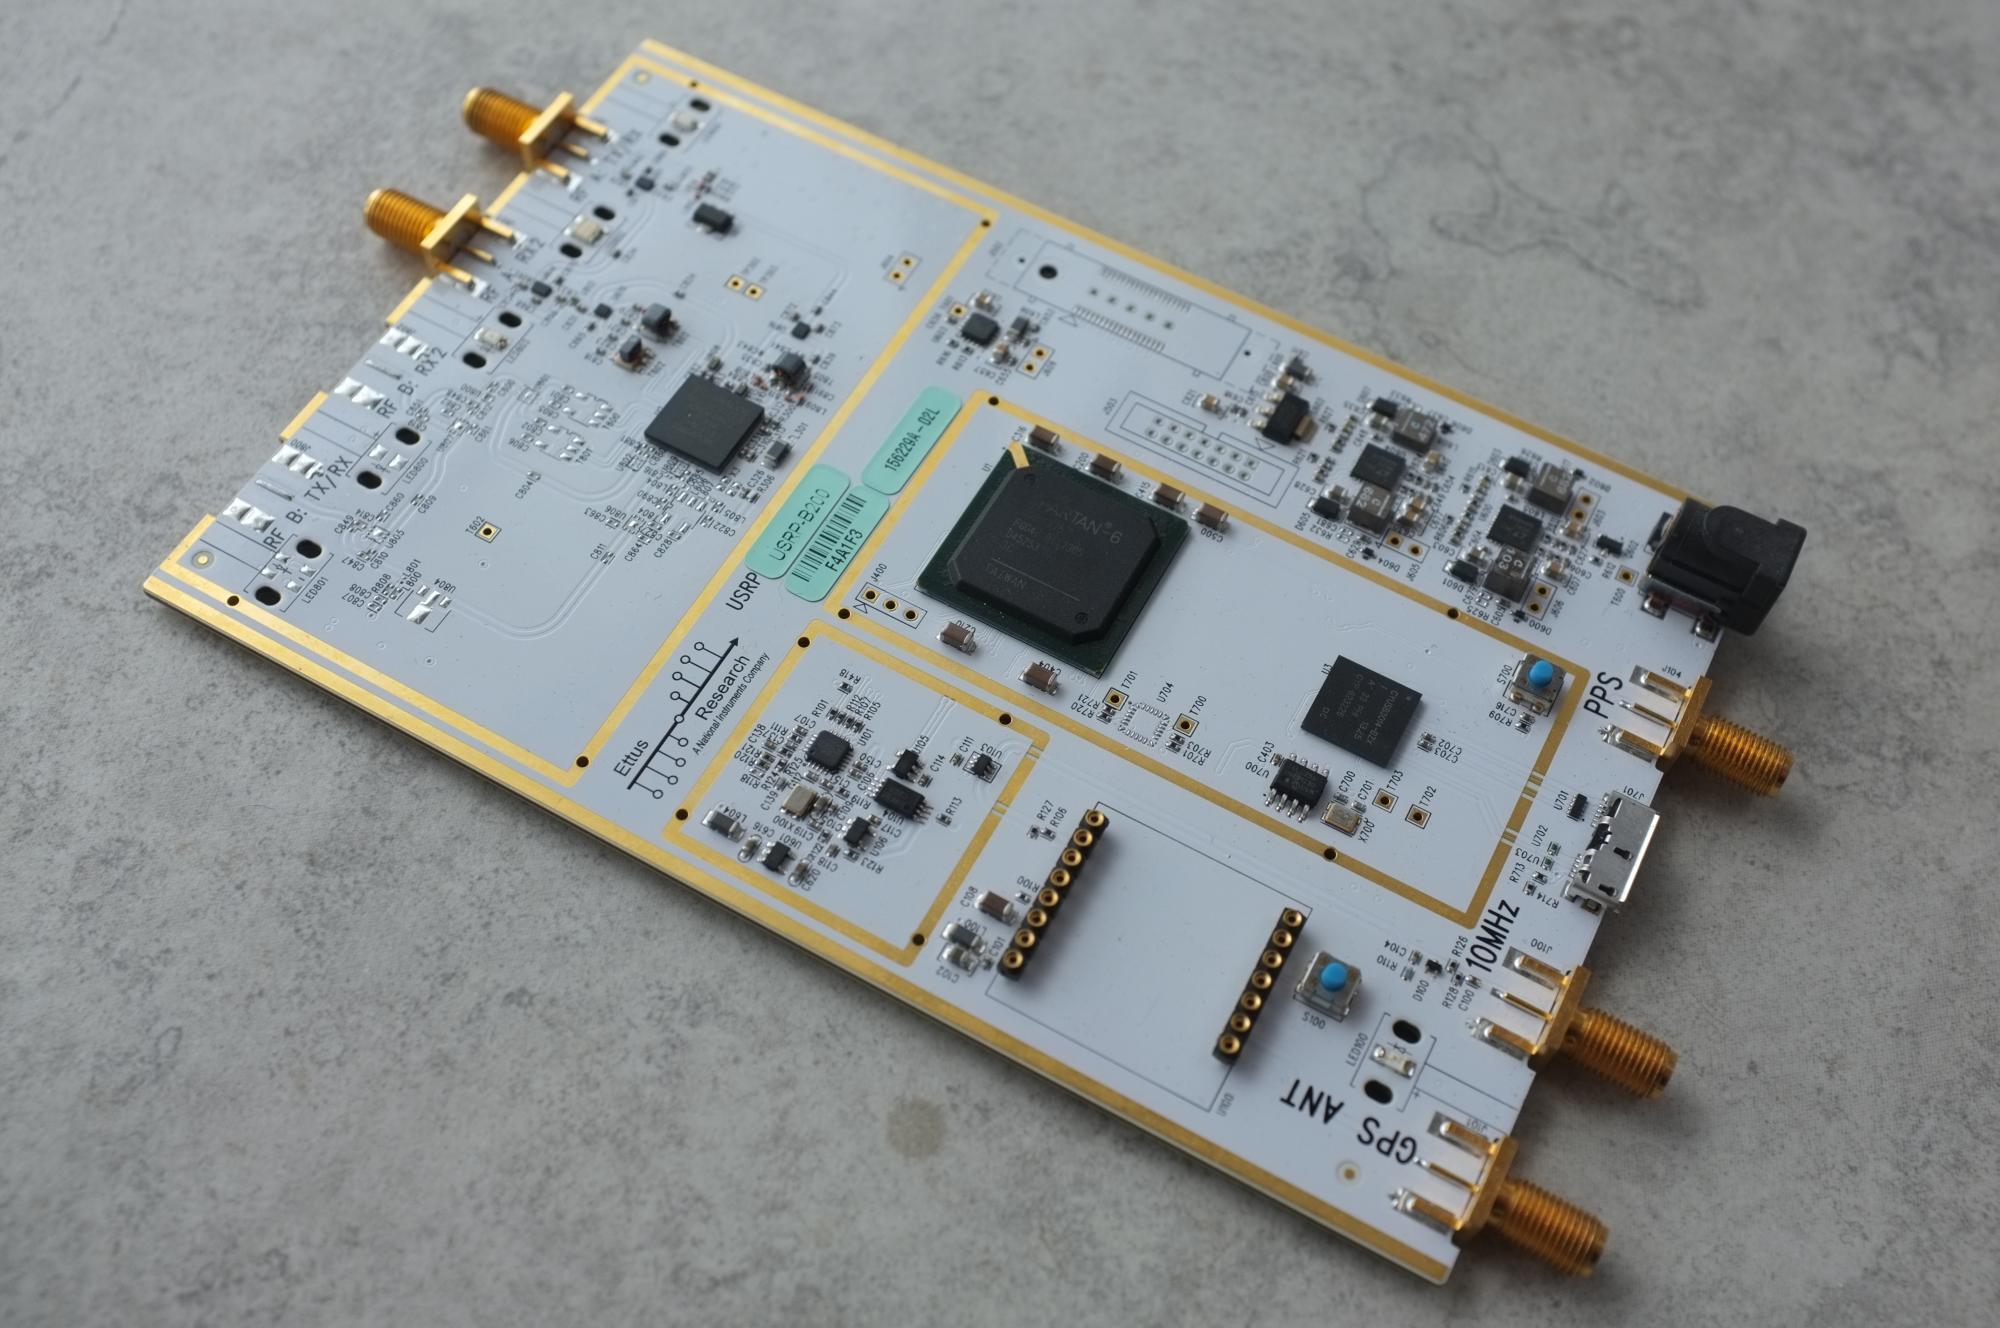
\includegraphics[width=12em]{figures/USRP-B200.jpg}
    \caption{Ettus USRP B200}
    \label{fig:usrp-b200}
\end{wrapfigure}


However, care has to be taken about the host system, especially about the USB
controller. Using USB~2.0 is not a problem for a DAB transmission, both USB~2.0
and USB~3.0 host controllers can therefore be used. Since USB~2.0 has been
around for longer and is more mature, it is sometimes preferable because it
causes less USB errors. This heavily depends on the exact model of the USB
controller inside the host PC, and has to be tested for each system.

The txgain on the B200 varies between $0$dB and about $90$dB. Experience shows
that compression effects begin to appear at values around $85$dB. This might be
different from device to device and needs to measured.

Similarly, the digital gain has to optimised for a given setting. It is
important that there is no digital clipping in the chain, because that leads to
problematic spurious spectrum components, that can disturb or even damage a
power amplifier.

There are some performance measurements available on the Opendigitalradio
wiki.\footnote{\url{http://wiki.opendigitalradio.org/index.php/USRP\_B200\_Measurements}}

\paragraph{Remarks concerning other USRP models}
We have used the USRP1, the USRP2 and the USRP B100 with the tools. The WBX is
the most appropriate daughterboard for these models.

The txgain setting has another range, it is best to start at $0$dB, and increase
it in steps of $3$dB or smaller while measuring the output signal, until the
correct power is reached.

\subsubsection{Other Hardware}
ODR-DabMod supports other radio interfaces using either standard output, or via
a fifo -- the latter must be created prior to runtime with the \texttt{mkfifo} command.
Due to limitations in the UHD driver library, \texttt{/dev/stdout} will only
function correctly if ODR-DabMod is configured at compilation time with the
following argument:

\begin{lstlisting}
--disable-output-uhd
\end{lstlisting}

ODR-DabMod has been tested working with HackRF from Great Scott Gadgets on i386 and
x86 architectures.\footnote{HackRF has not been tested to any degree of success
with ARM-based computers at this time as they are not (yet) capable of resampling
to the required higher rates as the process is highly CPU intensive.}

The unit is an entry level yet versatile SDR which provides coverage between
$\approx10$MHz to $6$GHz, and DAB signals been successfully generated with it in
VHF Band III ($174$--$240$MHz), L-Band ($1462$--$1467.5$MHz) and even the worldwide ISM
Band ($2400$--$2500$MHz). The latter (subject to local regulations) is a licence exempt
band which may be useful for performing freely radiating tests at low power. Cheap
MMDS converters are currently available which helpfully provide a Band III IF output
providing a direct feed to the aerial input of a receiver. Before choosing a converter
it is important to pay close attention to the specifications. The local oscillator
phase noise performance, and the dynamic range (due to the heavy use of the band) are
both particularly important.

To use HackRF, the output of ODR-DabMod must be set (in the configuration file) to
produce 8-bit signed integers, rather than the default complex floats.
HackRF has selectable baseband filters, however the lowest filter setting
($1.75$MHz) does not provide adequate image rejection at the native sampling rate of
$2048$k samples per second. An appropriate rate to start with is $4096$k, and for
some purposes this may well be adequate as this moves the image signals
generated within the radio far enough into the stop-band of filter to attenuate
them significantly. The digital gain in the ODR-DabMod configuration file should
be set to a maximum of $2.4$ at this rate to avoid digital clipping on modulation
peaks.

Example of the settings in the \texttt{mod.ini} file suitable for use with HackRF:

\begin{lstlisting}
[remotecontrol]
telnet=1
telnetport=2121

[input]
transport=file
source=myfirst.eti
loop=1

[modulator]
gainmode=2
digital_gain=2.4
rate=4096000

[firfilter]
enabled=1
filtertapsfile=filtertaps.txt

[output]
output=file

[fileoutput]
format=s8
filename=/tmp/ofdm.fifo

\end{lstlisting}

The output fifo has to be created beforehand, and the \texttt{hackrf\_transfer}
utility is then used to transmit the signal to the device.

Depending on the capabilities of the host computer, using higher sampling rates
($6144$k, and even $8192$k) may be possible. This oversampling is desirable as
it helps to produce a cleaner spectral output. At higher rates one needs to
ensure that samples are not being dropped on the USB and that CPU resources are
not being contended. It is also important to note that the digital gain value
must also be scaled accordingly as the sampling rate is increased. Two sets of
values are provided which reflect the theoretical values, and the second set
given in parentheses are empirical maximum values determined while monitoring
shoulder performance (measured at $970$kHz offset from the centre frequency)
using a spectrum analyser in $\approx 3$ kHz resolution bandwidth. The digital
gain figures for the tested sampling rates are shown below:

\begin{center}
\begin{tabular}{| l | c | c |}
    \hline
    Rate       & Dgain & Max Dgain (Empirical) \\ \hline \hline
    $4096$ksps & $2.0$ & $2.25$ \\ \hline
    $6144$ksps & $3.0$ & $3.37$ \\ \hline
    $8192$ksps & $4.0$ & $4.50$ \\
    \hline
\end{tabular}
\end{center}

The shoulder performance has been measured with shoulder performance at a little
better than $35$dB, which is roughly equivalent to that obtained from first
generation commercial modulator equipment. This can be increased to a relatively
respectable $\approx 40$dB by enabling the FIR baseband filter in ODR-DabMod,
and supplying it with an appropriate coefficient (tap) file. The maximum output
power available to mmet these performance figures is approximately $-10$dBm RMS.

Example of using ODR-DabMod with the \texttt{hackrf\_transfer} utility:

\begin{lstlisting}
mkfifo /tmp/ofdm.fifo
odr-dabmod mod.ini &
hackrf_transfer -t /tmp/ofdm.fifo -f 216928000 -x 47 \
    -a 1 -s 4096000 -b 1750000
\end{lstlisting}



\subsection{Audio Sources}
Preparing a DAB multiplex with different programmes requires that we are able to
read and encode several audio sources. We have seen in
section~\ref{sec:between_encoder_and_multiplexer} how the encoders can be
interfaced to the modulator. In this section we'll go through the different ways
to carry the audio data to the encoder.

\subsubsection{Local Audio Card}
It is possible to use an audio card connected to the computer as source. For
very simple scenarios, the ALSA input for FDK-AAC-DABplus is easiest to set up.
This however limits the usage of a single encoder per sound-card, and will not
scale well if more than one programme has to be encoded on the machine. It is
however ideal for dedicated encoding machines that can contribute the encoded
audio over an IP network.

An alternative to using ALSA is JACK\footnote{The JACK Audio Connection Kit is a
    virtual audio patch, \url{http://www.jack-audio.org}}
that can be used with a multi-channel sound card. JACK will expose every audio
input channel, and several encoders can be launched that also connect to JACK.
The input channels can be freely connected to the encoders thanks to the virtual
JACK patch panel.

\sidenote{It might be possible to use the libVLC input too, to be defined.}
FDK-AAC-DABplus supports JACK and ALSA input, but Toolame-dab supports only the
JACK input.

\subsubsection{Using Existing Web-Streams}
\label{usingexistingwebstreams}
One common scenario is to transmit radio stations that already are available as
web-radio streams. For simplicity, it makes sense to get these web streams,
which are most often encoded in mp3 and available through HTTP, decode them, and
use them as audio source for the DAB or \dabplus encoder.

The advantage of this approach is that the radio itself does not need to setup a
new infrastructure if the stream is of good quality. The main disadvantage is
that the audio is encoded twice, and this coding cascading degrades the audio
quality.

Often, web-streams are encoded in mp3 at $44100\Hz$ sample-rate, whereas DAB
is most often $48000\Hz$ or sometimes $32000\Hz$. A sample-rate conversion is
necessary in the stream decoder.

There are many different stream decoders, and gstreamer, mpg123 and mplayer have
been tested. By far the easiest way is to use the libVLC binding that can be
compiled for Toolame-dab and FDK-AAC-DABplus. This library has
the same features as the VLC audio player, but the audio data is directly passed
to the encoding routines. This allows the encoder to receive all network
sources VLC supports, not only HTTP web-streams but also less common setups
e.g.\ encoded audio inside multicast UDP MPEG-TS.
This is illustrated in ``Studio A'' in figure~\ref{fig:txchain-with-encoders}.

We have also achieved good results with mplayer, and the dab-scripts
repository\footnote{\url{http://github.com/Opendigitalradio/dab-scripts}}
contains the script \texttt{encode-jack.sh} that uses mplayer, and illustrates
how it is possible to encode a web-stream to \dabplus. JACK is used to
interconnect the stream decoder to the \dabplus encoder.
This is illustrated in ``Studio B''.

\begin{figure}[h]
    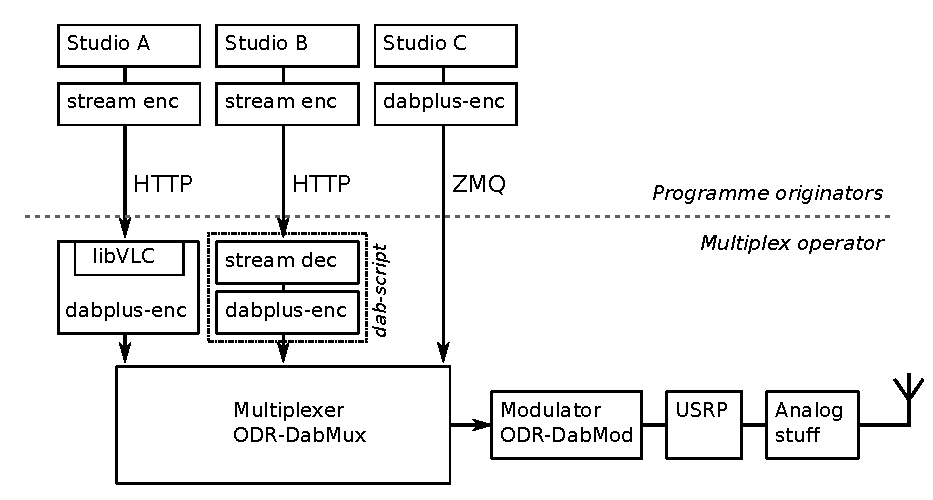
\includegraphics[width=\textwidth]{figures/txchain-with-encoders.pdf}
    \caption{Three common ways to encode a remote audio sources.}
    \label{fig:txchain-with-encoders}
\end{figure}


The scripts are designed for production use, and also contain automatic restart
logic in case of a failure. They send an email and write a message into the
system log.

\subsubsection{Encoders at Programme Originator Studios}
In order to avoid the unavoidable encoder cascading when using mp3 web-streams,
the DAB or \dabplus encoder has to be moved to the programme originator's
premises, and should directly encode the audio signal coming from the studios.
This is illustrated in ``Studio C'' in figure~\ref{fig:txchain-with-encoders}.

% vim: spl=en spell tw=80 et

% LICENSE: see LICENCE
\section{Data Features}
\subsection{FIG 1 Labels and FIG 2 Extended Labels}
The specification offers two ways to carry ensemble, service and component
labels: through FIG 1 and through FIG 2, specified in clauses 5.2.2.2 and 5.2.2.3
of ETSI EN 300 401~\cite{etsidab}.

Most receivers are only able to show FIG 1 Labels encoded in the Complete EBU
Latin character set (defined in ETSI TS 101 756 clause
5.2~\cite{etsidabtables}). Some are able to display Unicode FIG 1 Labels,
encoded either in UTF-8 or UCS-2, and, as of early 2019, receiver support for
FIG 2 Extended Labels is practically absent.

The main downside of carrying Unicode FIG 1 Labels is the length limitation: 16
bytes will only encode eight characters in alphabets that require two bytes per
character. FIG 2 supports up to 32 bytes labels to alleviate this.

The intention is that new ensembles in countries requiring labels in non-latin
alphabets transmit only FIG 2 Extended Labels, whereas currently operating
ensembles keep transmitting FIG 1 Labels. This entices receiver manufacturers to
support FIG 2 without impacting functionality of receivers currently in use.
Transmitting both FIG 1 and FIG 2 is discouraged by the specification.

The way FIG 2 is encoded has been redefined, which is why ODR-DabMux supports
two variants: FIG 2 with character flag being the old variant, and FIG 2 with
text control that will become the default variant.

\subsection{Announcements}
The ODR-DabMux multiplexer supports the insertion of FIG 0/18 and FIG 0/19 that
are used to define and trigger announcements according to ETSI TR 101 496-2
Clause 3.6.8~\cite{etsitr1014962}.
An example configuration is available in the ODR-DabMux repository, in
\texttt{doc/advanced.mux}.

The best known application for announcements is traffic information, but other
kinds of announcements can also be signalled. ODR-DabMux allows triggering the
announcements through the telnet and ZMQ remote control interfaces.

\subsection{Service Linking}
ODR-DabMux also supports the ability to inform receivers about other ways to
receive a given service, through the FIGs 0/6, 0/21 and 0/24. FIG 0/6
communicates the identifiers of services linked together, 0/21 informs the
receiver about other frequencies, and 0/24 includes information about other DAB
ensembles carrying the linked service.
Their interaction is outlined in ETSI TS 103 176~\cite{etsits103176}.

You will find an example configuration in the ODR-DabMux repository, in
\texttt{doc/servicelinking.mux}.

% vim: spl=en spell tw=80 et

% LICENSE: see LICENCE
\section{System Environment}

In this section, we describe the system configuration requirements for the
continuous operation of the tools. The production environment differs in some
respects to those used for experimentation and in laboratory testing. Monitoring,
automatic recovery (in case of errors) and resilience are crucial in 24/7
operations. The term \emph{production environment} will be used here to refer to
such use.

\subsection{Launching the tools}

Services running in a production environment are usually administered remotely,
and must be able to run without user intervention, or connection. Traditionally,
such services are implemented (in UNIX terminology) as `daemons'. These are
started and stopped using the init system contained within the distribution.
The ODR-mmbTools cannot daemonise themselves, so this requires another approach:

\paragraph{Screen multiplexer}
A simple approach is to use a screen multiplexer such as \emph{GNU Screen} or
\emph{tmux} - either of these can be used to launch a session from which the
user can detach, and later re-attach at will - leaving the tools running within
it. Please see the relevant manpages for more information.

Although a screen multiplexer alone permits the tools to run without a user
being connected, it alone cannot automatically restart failed processes, and it
is unable to provide warnings in the case of a problem.

The dab-scripts, already mentioned in \ref{usingexistingwebstreams}, can be
employed to monitor the processes and (if necessary) restart them, and send an
alert via email.

\paragraph{supervisord}
As an alternative to using the scripts, the execution of the tools can also be
carried out by a dedicated tool. \texttt{supervisor}\footnote{\url{http://supervisord.org}}
is (as the name implies) such a tool.

Once installed, supervisor reads its configuration file in \texttt{/etc/supervisor.conf}
and launches the processes that are to be monitored. Each process is described
by a file. The following example assumes the tools are run as user \texttt{odr},
and that the multiplex configuration is in \texttt{/home/odr/config.mux}, and
that ODR-DabMux is to be launched.The logs of ODR-DabMux is written to the
specified log files.

\begin{lstlisting}
[program:ODR-DabMux]
command=odr-dabmux config.mux
directory=/home/odr
user=odr
autostart=true
autorestart=true
stdout_logfile=/home/odr/logs/mux.out.log
stderr_logfile=/home/odr/logs/mux.err.log
\end{lstlisting}

Once this configuration has been added to the supervisor configuration, the
settings have to be re-read using:
\begin{lstlisting}
supervisorctl reread
\end{lstlisting}

In order for supervisor to start managing and running this process, it needs to
be added:

\begin{lstlisting}
supervisorctl add ODR-DabMux
\end{lstlisting}

Setting up more processes (such as any of the other tools) can be easily
achieved by customising the configuration template above. Examples are provided
in the \texttt{mmbtools-aux} repository, under the \texttt{supervisor} folder -
these need to be changed to reflect the paths that are in use on your system.

supervisor also includes a small web-server that can display the state of the
managed processes. It is enabled with the \verb+[inet_http_server]+ setting in
the configuration file.

\subsection{Logging}
Collecting information about events is essential within a production environment.
This information is essential forensic analysis, and tracing sources of trouble.
This is achieved through the logging of important messages that can be sent by
the tools.

ODR-DabMux and ODR-DabMod both support logging to standard error, to a file and
to the system logger \texttt{syslog}. Logging to syslog is the most flexible
approach; log information can be forwarded over the network to a
centralised logging server - where logs can then be filtered according to the
priority of each message. Both tools log to the LOCAL0 facility which in turn
can be redirected into an ODR-mmbtools specific log file.

\sidenote{Describe rsyslog configuration}

In order to avoid the log files from becoming undesirably large, \texttt{logrotate}
should be set to rotate the files automatically.

\sidenote{Describe logrotate configuration}


\subsection{Timing}
The ODR-mmbTools require the system time to be accurate in order for them to
function correctly - this is especially important when running a SFN, but is
also important for standalone transmitters when in a production environment. It
is also important to remember that most receivers have a clock that is
synchronised to the clock time which is being transmitted by the multiplex to
which it has been tuned.

The system needs to run a NTP client that synchronises the system time over the
network. Correct synchronisation can be checked using the \texttt{lpeers}
command of the \texttt{ntpq} tool. The magnitude of the offset should be below
$10$\ms.

The performance of the NTP synchronisation should also be monitored permanently
during operation.


\subsection{Monitoring using munin}

The Munin\footnote{\url{http://munin-monitoring.org/}} monitoring tool can
create graphs for essential system health parameters. It can also send emails
if values transgress the defined bounds - this assists the operator in the
assessment of system status, as well as the health of the services.

In addition to basic system measurements like CPU, RAM and disk usage, NTP
synchronisation, disk and network performance (and much more besides), there
are also custom data sources for ODR-DabMux.

These data sources include ZMQ input buffer monitoring (buffer level, underruns
and overruns) and the peak audio input levels (mono, or stereo). This
can be installed by copying \verb+doc/stats_dabmux_multi.py+ to
\texttt{/etc/munin/plugins.d}. They require that the ODR-DabMux management
server is enabled in the configuration, and will automatically generate the
graphs for the subchannels used in the configuration.


\subsection{Monitoring using Xymon}
The xymon monitoring tool\footnote{\url{http://xymon.sourceforge.net/}} is used
to monitor the health of many types of systems. It can present the results in
text, tables and/or graphs. It supports the basic health checks directly out of
the box, and can be extended with scripts to perform non-standard health checks.
The default mode of operation is that clients retrieve data and send it to the
xymon server, which interprets the results, displays them and generates alerts
if thresholds are exceeded. An alert can be send in an e-mail, an SMS or a
tweet.

The Perl script \verb+retodrs.pl+\footnote{The script name stands for
''Retrieve Opendigitalradio Status``}, retrieves the status and
statistics of an Opendigitalradio service and it reports the results to xymon.
The information is retrieved from the management server within ODR-DabMux. The
information presented includes a table with the status of each sub-channel and
the underrun and overrun rates on the sub-channels. If needed an alert can be
generated depending on the subchannel status or a rate exceeding a threshold.

The script needs to be installed on the same server running ODR-DABmux, as the
management service within it is only accessible from the same computer. This
implies that the xymon client software also needs to be installed on the same
machine. The client is configured to run the script.
The configuration and the scripts can typically be found in subdirectory
\verb+/usr/lib/xymon/client+, although that may depend on your distribution.

Once the client is set up, it needs to connect to a xymon server, which may or
may not be on the same machine.
The server is configured to limit the altering to specific sub-channels, to
store the statistical data and to generate graphs.
The configuration and the scripts on a xymon server are usually stored in the
subdirectory \verb+/usr/lib/xymon/server+.


\subsubsection{Installation of the Xymon Client}

The perl script has additional requirements:
\texttt{App::cpanminus}, \texttt{ZMQ::LibZMQ3}, and \texttt{JSON::PP}. They can
be installed through your distribution packages or using CPAN.

Once the script has been copied to \verb+/usr/lib/xymon/client/ext+, the
configuration of the launcher within the xymon client needs to be extended.
Create a new file named \verb+odrmux.cfg+ in
\verb+/usr/lib/xymon/client/etc/clientlaunch.d+ containing the following lines:

\begin{verbatim}
#
# Test odrmux checks the state and the statistics
# of the ODR-DabMux service.
#
[odrmux]
	ENVFILE $XYMONCLIENTHOME/etc/xymonclient.cfg
	CMD $XYMONCLIENTHOME/ext/retodrs.pl
	LOGFILE $XYMONCLIENTLOGS/retodrs.plog
	INTERVAL 5m
\end{verbatim}

After a restart of the xymon client, the script \verb+retodrs.pl+ will
be invoked once every 5 minutes.


\subsubsection{Server Configuration}

By default all subchannels will be monitored, and will raise alerts if the
status or the statistics are in outside of a valid operational range. The
alerting can be limited to a subset of the sub-channels by adding a tag to the
hosts-entry in the configuration file \verb+/usr/lib/xymon/server/etc/hosts.cfg+.
The additional tag is:

\begin{verbatim}
	ODR:select(<SubChannelName0>;<SubChannelName1>;...)
\end{verbatim}

The sub-channels not named will still be shown, but no alerts will be generated
for those sub-channels. This is visible as the green/yellow/red icons are
missing for those sub-channels.

Six statistic values are gathered by the script, namely
\texttt{BufferMin}, \texttt{BufferMax}, \texttt{PeakLeft}, \texttt{PeakRight},
\texttt{UnderRun} and \texttt{OverRun}. It is found that only the latter two
seem to contain sensible values all the time, so those values are the only
ones shown in a graph. Note that those values retrieved by the script are
ever-increasing counters, showing the total number of over-runs or under-runs.
In the graph, the average number of over-runs or under-runs per second, averaged
over a period of 5 minutes, is shown.

The first step is to have the collected statistics to be moved into a database,
a so-called \textit{Round Robin Database}. This is accomplished by adding a file
named \verb+odr.cfg+ in \verb+/usr/lib/xymon/server/etc/xymonserver.d+
containing the following lines:

\begin{verbatim}
TEST2RRD+=",odr_mux=devmon"
GRAPHS+=",odr_mux::1"
\end{verbatim}

The next step is to define the layout of the graph.
Create a file named \verb+graphs.odr.cfg+ in
\verb+/usr/lib/xymon/server/etc/graphs.d+ containing the following lines:

\begin{verbatim}
#
# Graphs to show the statistics collected from an
# Opendigitalradio DabMux server.
#
[odr_mux]
	FNPATTERN ^odr_mux\.(.+)\.rrd$
	TITLE , Frame loss rate
	YAXIS Rate [/s]
	-l 0
	DEF:ur@RRDIDX@=@RRDFN@:Underrun:AVERAGE
	DEF:or@RRDIDX@=@RRDFN@:Overrun:AVERAGE
	LINE1:ur@RRDIDX@#FF0000:@RRDPARAM@ underrun
	GPRINT:ur@RRDIDX@:MIN:Min \: %5.1lf %s
	GPRINT:ur@RRDIDX@:MAX:Max \: %5.1lf %s
	GPRINT:ur@RRDIDX@:AVERAGE:Avg \: %5.1lf %s
	GPRINT:ur@RRDIDX@:LAST:Cur \: %5.1lf %s\n
	LINE1:or@RRDIDX@#00FF00:@RRDPARAM@ overrun
	GPRINT:or@RRDIDX@:MIN: Min \: %5.1lf %s
	GPRINT:or@RRDIDX@:MAX:Max \: %5.1lf %s
	GPRINT:or@RRDIDX@:AVERAGE:Avg \: %5.1lf %s
	GPRINT:or@RRDIDX@:LAST:Cur \: %5.1lf %s\n
\end{verbatim}


\subsection{Real-time Scheduling}

As a general principle, it is prudent not to run tools (that do not need superuser
privileges) as the \texttt{root} user. The same principle also applies to the
ODR-mmbTools, but care has to be taken that the tools can still request real-time
scheduling when it is needed.

This is achieved by adding the following to \texttt{/etc/security/limits.conf},
assuming the tools are run under the user \texttt{odr}.

\begin{lstlisting}
odr          -       rtprio          65
odr          -       nice           -10
\end{lstlisting}

If you have installed JACK with real-time privileges, you may find this has
already been configured for the `audio' group, written as \texttt{@audio}, which
should suffice providing your desired user is a member of the `audio' group.

\subsection{Accessing the USRP as Non-root}

Superuser privileges are not required to access USB-connected USRP devices, but
sometimes the system lacks the configuration to enable normal users to
communicate with the device.
In that case, it is necessary to add a rule file for \texttt{udev}. This file is
included in the UHD sources, but might not have been automatically installed.
The file is called \texttt{10-uhd-usrp.rules}, should be placed into
\texttt{/etc/udev/rules.d/} and should contain

{ \footnotesize
\begin{verbatim}
#USRP1
SUBSYSTEMS=="usb", ATTRS{idVendor}=="fffe", ATTRS{idProduct}=="0002", MODE:="0666"
#B100
SUBSYSTEMS=="usb", ATTRS{idVendor}=="2500", ATTRS{idProduct}=="0002", MODE:="0666"
#B200
SUBSYSTEMS=="usb", ATTRS{idVendor}=="2500", ATTRS{idProduct}=="0020", MODE:="0666"
\end{verbatim}
}

% vim: spl=en spell tw=80 et

\section{Single-Frequency Networks}
\subsection{Requirements}
The DAB standard has been designed to enable the creation of transmission
networks where several transmitters share the same frequency, and send the same
signal synchronously. Such networks are called ``Single-Frequency Networks''.
Each transmitter needs to be fed the same multiplex stream, which must include
timing information required for synchronisation. This timing information implies
that a time reference must be installed at each transmitter.

The requirements for a SFN can therefore be summarised in three points:
\begin{itemize}
    \item The signal must be \emph{identical} for each transmitter. This
        requires a common multiplexers, and a distribution network that carries
        the ETI to all modulators.
    \item All transmitters must transmit on the \emph{same frequency}. The modulators
        require a frequency reference.
    \item The signal must be transmitted at the \emph{same time}, which requires
        a time reference at each site. It also implies that the ETI stream must
        contain timestamps.
\end{itemize}


The figure~\ref{fig:txchain-sfn} shows a SFN setup with two transmitters.

\begin{figure}[h]
    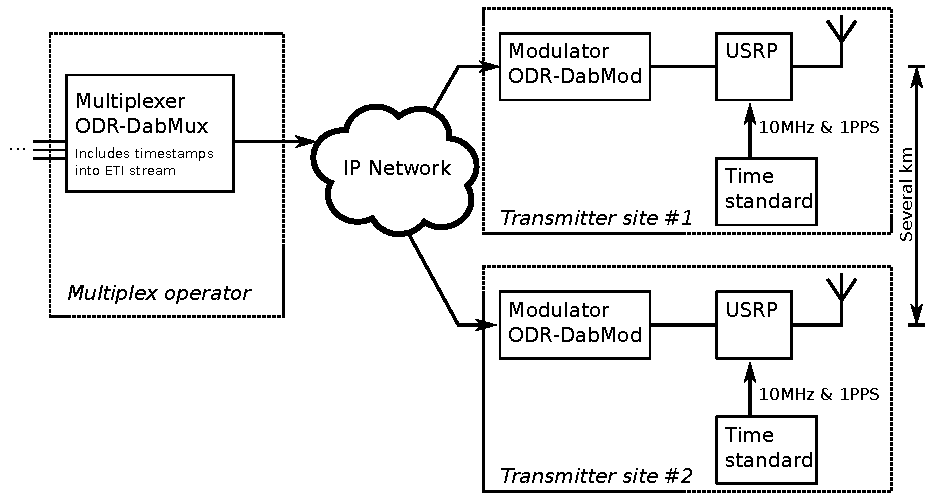
\includegraphics[width=\textwidth]{figures/txchain-sfn.pdf}
    \caption{This outline for a SFN shows two transmission sites.}
    \label{fig:txchain-sfn}
\end{figure}

\sidenote{Explain requirements on system time, NTP}

\subsection{Multiplexer Configuration}
On the ODR-DabMux configuration, there are not many options that are specific to
an SFN setup.
Most importantly, the timestamp feature must be enabled using the ``tist'' option in
the ``general'' section.

Furthermore, it is recommended to use the ZeroMQ transport between the
multiplexer and the modulators, which can be enabled in the ``outputs'' section.
Care has to be taken to have an output that slows ODR-DabMux down to nominal
rate. The ZeroMQ output alone does not enforce this. The following listing shows
the relevant options we just covered.

\begin{lstlisting}
general {
    tist true
    ...
}

...

outputs {
    ; Accept connections on all interfaces, on port 9100
    zmq  "zmq+tcp://*:9100"
    ; This throttles muxing down to nominal rate
    throttle "simul://"
}
\end{lstlisting}

\subsection{Modulator Configuration}
Since the modulator has to ensure that the three SFN requirements are satisfied,
its configuration is more complex.

We will assume, in this explanation, that one of the following USRP devices is
used: USRP2, USRP B100, USRP B200. Other devices also support the necessary time
and frequency synchronisation, but they have not been well tested. These USRP
devices can accept different sources for the reference clock:
\begin{itemize}
    \item The default ``internal'' source uses the non-disciplined
        clock generator inside the USRP. It is not suitable for SFN.
    \item The ``external'' source corresponds to the SMA connector on
        the USRP. A 10MHz signal from an external source must be connected to
        it.
    \item The optional GPSDO that can be mounted inside the USRP, and is
        selected as source with the ``gpsdo'' setting.
\end{itemize}

For the time reference, the ``pps\_source'' option is used. Possible values are
``none'', ``external'' and ``gpsdo'', with analogous meaning as for the
reference clock.

In case the USRP is connected to external references, the relevant configuration
would be as follows:

\begin{lstlisting}
[uhdoutput]
refclk_source=external
pps_source=external
\end{lstlisting}

These settings alone do not tell the modulator to enable synchronisation of the
transmission, they only select how the USRP is configured. To enable timestamp
decoding and the frame synchronisation logic in ODR-DabMod, the following
settings must also be set:

\begin{lstlisting}
[delaymanagement]
synchronous=1

; The constant offset to be added to the TIST, in seconds
offset=2.0
\end{lstlisting}

The ``offset'' setting deserves some further explanations. The ETI data stream
contains TIST information, from which a time-stamp for each ETI frame can be
derived. Each ETI frame ($24$\ms interval) is therefore associated with a
precise point in time that defines the time of transmission of the corresponding
transmission frame.\footnote{It is slightly more complex, because one
    transmission frame is composed of several ETI frames in some
    transmission modes, but the principle stays the same. It suffices for this
    explanation that we can derive the transmission time from the TIST
information.} The TIST information is set to current time at ETI frame
generation, and does not take in account the propagation delay across the
distribution network. Therefore, we need to add an offset, called $\delta$, to
the TIST to define transmission time.

\[
t_{transmission} = t_{TIST} + \delta
\]

If this offset is set to a higher value, there will be a bigger delay (measured
in absolute time) between the point in time a frame is multiplexed and the point
in time the frame is transmitted. More frames therefore will be buffered in
the ODR-DabMod ZeroMQ input, increasing robustness against network latency
fluctuations.

The offset already has two functions: it compensates for network delay and
allows a trade-off between delay and robustness. But it also serves a third
purpose: When doing coverage planning for an SFN, it is necessary to be able to
control the relative delay between transmitters in the order of milliseconds.
This tuning of relative delay is included in the ``offset'' setting. We can
therefore rewrite the above equation as:

\[
    t_{transmission} = t_{TIST} + \delta_{network} + \delta_{planning}
\]
\[
    \delta = \delta_{network} + \delta_{planning}
\]

\sidenote{Explain relationship with ZeroMQ max buffer size}

\subsection{Using ODR LEA-M8F GPSDO board}

The ODR GPSDO board integrating a u-blox LEA-M8F module can be used as time and
frequency reference for the USRP B200. \sidenote{TODO: Add Picture}
The board design is available on the Opendigitalradio website, with
a bill of materials describing how to source the components. The PCB itself can
be manufactured in any PCB fab.

The module includes the correct pin header so that it can be mounted directly
onto the USRP B200, but also includes footprints for SMA connectors for other
usages. Communication between the PC and the GPS is possible through USB or over
UART through the B200.

The u-blox LEA-M8F module is a GPS disciplined TCXO module, with a one-pulse per
second and a reference clock output at a frequency of $30.72$ MHz. This is
different than what the normal USRP firmware expects.

Because the UART communication protocol and the reference clock frequency are
different than for the GPSDO units Ettus supports, a modified version of UHD is
necessary. This version includes new UHD sensors, used by ODR-DabMod to verify
that the GPSDO is locked properly, and different configuration settings for the
clock management PLL inside the USRP, making the USRP compatible to the
$30.72$MHz reference clock frequency.

The modified UHD version is available at
\url{http://www.github.com/Opendigitalradio/uhd.git} and replaces Ettus' UHD.

ODR-DabMod can be configured as follows:
\begin{lstlisting}
[uhdoutput]
refclk_source=gpsdo
pps_source=gpsdo
behaviour_refclk_lock_lost=crash
max_gps_holdover_time=600
\end{lstlisting}


\subsection{Using Ettus GPSDO}

\sidenote{Give example}

% vim: spl=en spell tw=80 et

\appendix
% LICENSE: see LICENCE

\section{ODR-DabMux ETI file formats}
\label{etiformat}
ODR-DabMux supports three output formats for the ETI stream, that have been described on the mmbTools forum
website.\footnote{\url{http://mmbtools.crc.ca/component/option,com\_fireboard/Itemid,55/func,view/id,4/catid,13/\#28}}

The three formats are called \emph{framed}, \emph{streamed} and \emph{raw}.

The \emph{framed} format is used for saving a finite ETI stream into a file. Each frame does not contain any padding, and the
format can be described as follows:
\begin{lstlisting}
uint32_t nbFrames
// for each frame
  uint16_t frameSize
  uint8_t data[frameSize]
\end{lstlisting}

When streaming data, in which case the number of frames is not known in advance, the \emph{streamed} format can be used.
This format is identical to the first one except for the missing \texttt{nbFrames}.
\begin{lstlisting}
// for each frame
  uint16_t frameSize
  uint8_t data[frameSize]
\end{lstlisting}

The \emph{raw} format corresponds to ETI(NI), where each frame has a constant size of 6144 Bytes. The padding in this
case is necessary.
\begin{lstlisting}
// for each frame
  uint8_t data[6144]
\end{lstlisting}

In order to select the format, the following syntax for the \texttt{-O} option is used:
\texttt{-O file://filename?type=format}, where \texttt{format} is one of \verb+framed+, \verb+streamed+ or
\verb+raw+.


\section{Additional EDI TAGs used}
ODR defined and uses two additional EDI TAGs, whose content is described here.

ODR-AudioEnc inserts audio level metadata into the ``ODRa'' TAG. The TAG item is in the following format:
\begin{lstlisting}
  TAG Name="ODRa" [4 bytes]
  Length=4 [4 bytes]
  Left Audio Level [signed 16-bit integer]
  Right Audio Level [signed 16-bit integer]
\end{lstlisting}


The second EDI TAG ``ODRv'' contains version and uptime information for the EDI source.
\begin{lstlisting}
  TAG Name="ODRv" [4 bytes]
  Length=N+4 [4 bytes]
  Version [String of N bytes, UTF-8 encoded, not zero terminated]
  Uptime [unsigned 32-bit integer representing number of seconds since program start]
\end{lstlisting}


\section{Bibliography}
\bibliographystyle{acm}
\bibliography{dab}



\end{document}

% vim: spl=en spell tw=80 et
